\section{Pontos de decisão}

Uma funcionalidade muito comum em sistemas Web é poder definir a mudança de fluxo de telas por meio de código, ou seja, a mudança depende de um resultado de um dado ou ação prévia. Para tal, existe um mecanismo dentro da UML chamados Pontos de Decisão para modelar esse semântica.

Nela você desenha uma linha de transição a partir da ação conectando-a ao ponto
de decisão. Um ponto de decisão é desenhado como um losango em UML. Já que uma
decisão tem pelo menos dois resultados diferentes, o ponto de decisão terá
múltiplas transições para diferentes ações.

Usaremos como exemplo para introduzir um ponto de decisão o seguinte diagrama de
atividades:

\begin{figure}[H]
	\centering
	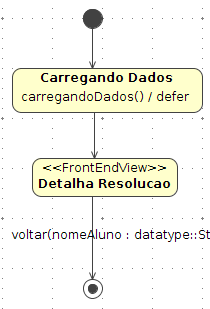
\includegraphics[scale=0.75]{files/imgs/decision-point-00.png}
	\caption{Modelo inicial do exemplo}
	\label{modelo_inicial_ponto_decisao}
\end{figure}

Criamos um ponto de decisão e colocamos uma transição do estado
\textbf{Carregando Dados} para o ponto de decisão:

\begin{figure}[H]
	\centering
	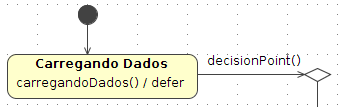
\includegraphics[scale=0.75]{files/imgs/decision-point-01.png}
	\caption{Criando o ponto de decisão}
	\label{criando_ponto_decisao}
\end{figure}

Em seguida na classe de controle do diagrama de atividades criamos uma função
chamada \texttt{decisionPoint}:

\begin{figure}[H]
	\centering
	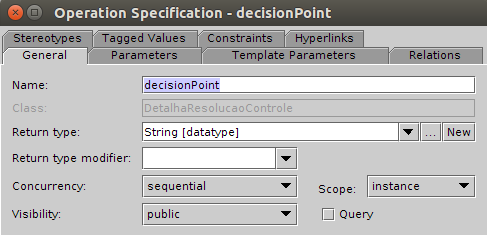
\includegraphics[scale=0.75]{files/imgs/decision-point-02.png}
	\caption{Criando função do ponto de decisão}
	\label{funcao_ponto_decisao}
\end{figure}

Na transição para o ponto de decisão, alteramos a \texttt{trigger} e colocamos o
tipo dela como \texttt{call} e a operação como \texttt{decisionPoint}:

\begin{figure}[H]
	\centering
	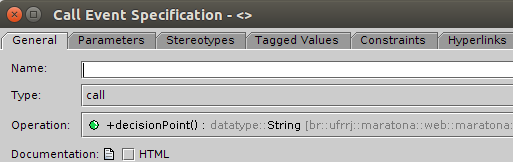
\includegraphics[scale=0.75]{files/imgs/decision-point-03.png}
	\caption{Colocando a função na transição}
	\label{funcao_transicao}
\end{figure}

O próximo passo é passar o início da transição que ia de \textbf{Carregando
Dados} para \textbf{Detalha Resolucao} para o ponto de decisão e criar uma
transição do ponto de decisão para o estado final.

\begin{figure}[H]
	\centering
	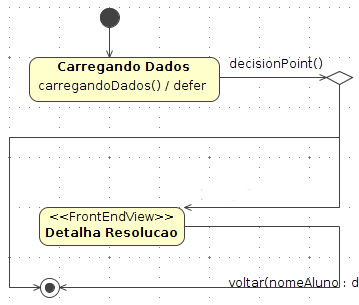
\includegraphics[scale=0.75]{files/imgs/decision-point-04.png}
	\caption{Colocando a função na transição}
	\label{ponto_decisao_com_transicoes}
\end{figure}

Em seguida devemos criar a condição de guarda dessas transições. Na aba
\texttt{General}, clicamos no botão \texttt{Edit} da seção \texttt{Guard}:

\begin{figure}[H]
	\centering
	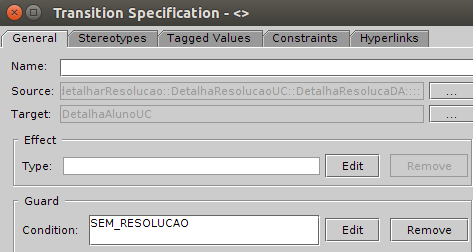
\includegraphics[scale=0.75]{files/imgs/decision-point-05.png}
	\caption{Abrindo a transição}
	\label{abrindo_transição}
\end{figure}

Agora especificamos o nome da condição de guarda e a condição em si. Ambos tem
que ter o mesmo nome:

\begin{figure}[H]
	\centering
	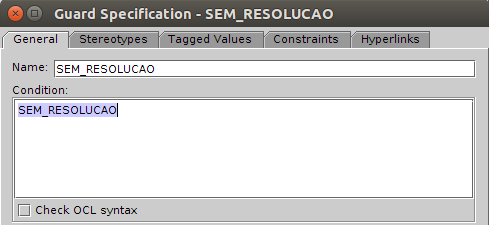
\includegraphics[scale=0.75]{files/imgs/decision-point-06.png}
	\caption{Especificando a condição de guarda}
	\label{condicao_de_guarda}
\end{figure}

Fazemos o mesmo para a outra transição e o modelo final é o seguinte:

\begin{figure}[H]
	\centering
	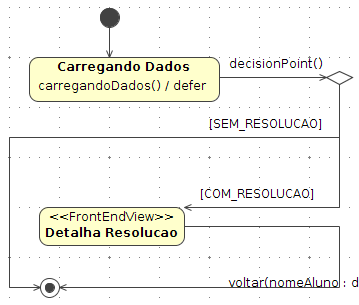
\includegraphics[scale=0.75]{files/imgs/decision-point-07.png}
	\caption{Modelo final}
	\label{modelo_final}
\end{figure}

Agora temos que implementar a função \texttt{decisionPoint}. Ela tem que
retornar uma String que seja uma das condições de guarda especificadas no
modelo. Exemplo de código:

\begin{lstlisting}[language=java, frame=single, breaklines=true]
	public String decisionPoint(DecisionPointForm form, ViewContainer container) throws Exception
	{
		if (form.getIdResolucao() != null) {
			return "COM_RESOLUCAO";
		}
		else {
			return "SEM_RESOLUCAO";
		}
	}
\end{lstlisting}